\documentclass[1p]{elsarticle_modified}
%\bibliographystyle{elsarticle-num}

%\usepackage[colorlinks]{hyperref}
%\usepackage{abbrmath_seonhwa} %\Abb, \Ascr, \Acal ,\Abf, \Afrak
\usepackage{amsfonts}
\usepackage{amssymb}
\usepackage{amsmath}
\usepackage{amsthm}
\usepackage{scalefnt}
\usepackage{amsbsy}
\usepackage{kotex}
\usepackage{caption}
\usepackage{subfig}
\usepackage{color}
\usepackage{graphicx}
\usepackage{xcolor} %% white, black, red, green, blue, cyan, magenta, yellow
\usepackage{float}
\usepackage{setspace}
\usepackage{hyperref}

\usepackage{tikz}
\usetikzlibrary{arrows}

\usepackage{multirow}
\usepackage{array} % fixed length table
\usepackage{hhline}

%%%%%%%%%%%%%%%%%%%%%
\makeatletter
\renewcommand*\env@matrix[1][\arraystretch]{%
	\edef\arraystretch{#1}%
	\hskip -\arraycolsep
	\let\@ifnextchar\new@ifnextchar
	\array{*\c@MaxMatrixCols c}}
\makeatother %https://tex.stackexchange.com/questions/14071/how-can-i-increase-the-line-spacing-in-a-matrix
%%%%%%%%%%%%%%%

\usepackage[normalem]{ulem}

\newcommand{\msout}[1]{\ifmmode\text{\sout{\ensuremath{#1}}}\else\sout{#1}\fi}
%SOURCE: \msout is \stkout macro in https://tex.stackexchange.com/questions/20609/strikeout-in-math-mode

\newcommand{\cancel}[1]{
	\ifmmode
	{\color{red}\msout{#1}}
	\else
	{\color{red}\sout{#1}}
	\fi
}

\newcommand{\add}[1]{
	{\color{blue}\uwave{#1}}
}

\newcommand{\replace}[2]{
	\ifmmode
	{\color{red}\msout{#1}}{\color{blue}\uwave{#2}}
	\else
	{\color{red}\sout{#1}}{\color{blue}\uwave{#2}}
	\fi
}

\newcommand{\Sol}{\mathcal{S}} %segment
\newcommand{\D}{D} %diagram
\newcommand{\A}{\mathcal{A}} %arc


%%%%%%%%%%%%%%%%%%%%%%%%%%%%%5 test

\def\sl{\operatorname{\textup{SL}}(2,\Cbb)}
\def\psl{\operatorname{\textup{PSL}}(2,\Cbb)}
\def\quan{\mkern 1mu \triangleright \mkern 1mu}

\theoremstyle{definition}
\newtheorem{thm}{Theorem}[section]
\newtheorem{prop}[thm]{Proposition}
\newtheorem{lem}[thm]{Lemma}
\newtheorem{ques}[thm]{Question}
\newtheorem{cor}[thm]{Corollary}
\newtheorem{defn}[thm]{Definition}
\newtheorem{exam}[thm]{Example}
\newtheorem{rmk}[thm]{Remark}
\newtheorem{alg}[thm]{Algorithm}

\newcommand{\I}{\sqrt{-1}}
\begin{document}

%\begin{frontmatter}
%
%\title{Boundary parabolic representations of knots up to 8 crossings}
%
%%% Group authors per affiliation:
%\author{Yunhi Cho} 
%\address{Department of Mathematics, University of Seoul, Seoul, Korea}
%\ead{yhcho@uos.ac.kr}
%
%
%\author{Seonhwa Kim} %\fnref{s_kim}}
%\address{Center for Geometry and Physics, Institute for Basic Science, Pohang, 37673, Korea}
%\ead{ryeona17@ibs.re.kr}
%
%\author{Hyuk Kim}
%\address{Department of Mathematical Sciences, Seoul National University, Seoul 08826, Korea}
%\ead{hyukkim@snu.ac.kr}
%
%\author{Seokbeom Yoon}
%\address{Department of Mathematical Sciences, Seoul National University, Seoul, 08826,  Korea}
%\ead{sbyoon15@snu.ac.kr}
%
%\begin{abstract}
%We find all boundary parabolic representation of knots up to 8 crossings.
%
%\end{abstract}
%\begin{keyword}
%    \MSC[2010] 57M25 
%\end{keyword}
%
%\end{frontmatter}

%\linenumbers
%\tableofcontents
%
\newcommand\colored[1]{\textcolor{white}{\rule[-0.35ex]{0.8em}{1.4ex}}\kern-0.8em\color{red} #1}%
%\newcommand\colored[1]{\textcolor{white}{ #1}\kern-2.17ex	\textcolor{white}{ #1}\kern-1.81ex	\textcolor{white}{ #1}\kern-2.15ex\color{red}#1	}

{\Large $\underline{12a_{0971}~(K12a_{0971})}$}

\setlength{\tabcolsep}{10pt}
\renewcommand{\arraystretch}{1.6}
\vspace{1cm}\begin{tabular}{m{100pt}>{\centering\arraybackslash}m{274pt}}
\multirow{5}{120pt}{
	\centering
	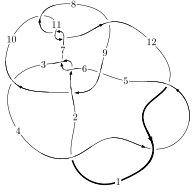
\includegraphics[width=112pt]{../../../GIT/diagram.site/Diagrams/png/1772_12a_0971.png}\\
\ \ \ A knot diagram\footnotemark}&
\allowdisplaybreaks
\textbf{Linearized knot diagam} \\
\cline{2-2}
 &
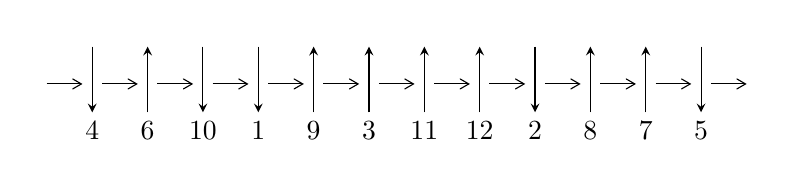
\begin{tikzpicture}[x=20pt, y=17pt]
	% nodes
	\node (C0) at (0, 0) {};
	\node (C1) at (1, 0) {};
	\node (C1U) at (1, +1) {};
	\node (C1D) at (1, -1) {4};

	\node (C2) at (2, 0) {};
	\node (C2U) at (2, +1) {};
	\node (C2D) at (2, -1) {6};

	\node (C3) at (3, 0) {};
	\node (C3U) at (3, +1) {};
	\node (C3D) at (3, -1) {10};

	\node (C4) at (4, 0) {};
	\node (C4U) at (4, +1) {};
	\node (C4D) at (4, -1) {1};

	\node (C5) at (5, 0) {};
	\node (C5U) at (5, +1) {};
	\node (C5D) at (5, -1) {9};

	\node (C6) at (6, 0) {};
	\node (C6U) at (6, +1) {};
	\node (C6D) at (6, -1) {3};

	\node (C7) at (7, 0) {};
	\node (C7U) at (7, +1) {};
	\node (C7D) at (7, -1) {11};

	\node (C8) at (8, 0) {};
	\node (C8U) at (8, +1) {};
	\node (C8D) at (8, -1) {12};

	\node (C9) at (9, 0) {};
	\node (C9U) at (9, +1) {};
	\node (C9D) at (9, -1) {2};

	\node (C10) at (10, 0) {};
	\node (C10U) at (10, +1) {};
	\node (C10D) at (10, -1) {8};

	\node (C11) at (11, 0) {};
	\node (C11U) at (11, +1) {};
	\node (C11D) at (11, -1) {7};

	\node (C12) at (12, 0) {};
	\node (C12U) at (12, +1) {};
	\node (C12D) at (12, -1) {5};
	\node (C13) at (13, 0) {};

	% arrows
	\draw[->,>={angle 60}]
	(C0) edge (C1) (C1) edge (C2) (C2) edge (C3) (C3) edge (C4) (C4) edge (C5) (C5) edge (C6) (C6) edge (C7) (C7) edge (C8) (C8) edge (C9) (C9) edge (C10) (C10) edge (C11) (C11) edge (C12) (C12) edge (C13) ;	\draw[->,>=stealth]
	(C1U) edge (C1D) (C2D) edge (C2U) (C3U) edge (C3D) (C4U) edge (C4D) (C5D) edge (C5U) (C6D) edge (C6U) (C7D) edge (C7U) (C8D) edge (C8U) (C9U) edge (C9D) (C10D) edge (C10U) (C11D) edge (C11U) (C12U) edge (C12D) ;
	\end{tikzpicture} \\
\hhline{~~} \\& 
\textbf{Solving Sequence} \\ \cline{2-2} 
 &
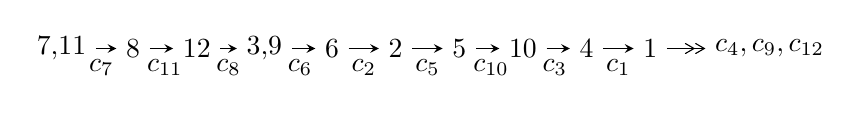
\begin{tikzpicture}[x=23pt, y=7pt]
	% node
	\node (A0) at (-1/8, 0) {7,11};
	\node (A1) at (1, 0) {8};
	\node (A2) at (2, 0) {12};
	\node (A3) at (49/16, 0) {3,9};
	\node (A4) at (33/8, 0) {6};
	\node (A5) at (41/8, 0) {2};
	\node (A6) at (49/8, 0) {5};
	\node (A7) at (57/8, 0) {10};
	\node (A8) at (65/8, 0) {4};
	\node (A9) at (73/8, 0) {1};
	\node (C1) at (1/2, -1) {$c_{7}$};
	\node (C2) at (3/2, -1) {$c_{11}$};
	\node (C3) at (5/2, -1) {$c_{8}$};
	\node (C4) at (29/8, -1) {$c_{6}$};
	\node (C5) at (37/8, -1) {$c_{2}$};
	\node (C6) at (45/8, -1) {$c_{5}$};
	\node (C7) at (53/8, -1) {$c_{10}$};
	\node (C8) at (61/8, -1) {$c_{3}$};
	\node (C9) at (69/8, -1) {$c_{1}$};
	\node (A10) at (11, 0) {$c_{4},c_{9},c_{12}$};

	% edge
	\draw[->,>=stealth]	
	(A0) edge (A1) (A1) edge (A2) (A2) edge (A3) (A3) edge (A4) (A4) edge (A5) (A5) edge (A6) (A6) edge (A7) (A7) edge (A8) (A8) edge (A9) ;
	\draw[->>,>={angle 60}]	
	(A9) edge (A10);
\end{tikzpicture} \\ 

\end{tabular} \\

\footnotetext{
The image of knot diagram is generated by the software ``\textbf{Draw programme}" developed by Andrew Bartholomew(\url{http://www.layer8.co.uk/maths/draw/index.htm\#Running-draw}), where we modified some parts for our purpose(\url{https://github.com/CATsTAILs/LinksPainter}).
}\phantom \\ \newline 
\centering \textbf{Ideals for irreducible components\footnotemark of $X_{\text{par}}$} 
 
\begin{align*}
I^u_{1}&=\langle 
3.15928\times10^{85} u^{86}-7.95197\times10^{85} u^{85}+\cdots+1.03342\times10^{86} b-3.69881\times10^{86},\\
\phantom{I^u_{1}}&\phantom{= \langle  }1.34443\times10^{86} u^{86}-4.14253\times10^{86} u^{85}+\cdots+9.30081\times10^{86} a-2.18852\times10^{87},\;u^{87}-3 u^{86}+\cdots-13 u+9\rangle \\
I^u_{2}&=\langle 
45 u^2 a+18 a u+15 u^2+7 b+75 a+6 u+25,\;3 u^2 a+3 a^2+3 a u-3 u^2+3 a-6 u-2,\;u^3+u^2+2 u+1\rangle \\
\\
\end{align*}
\raggedright * 2 irreducible components of $\dim_{\mathbb{C}}=0$, with total 93 representations.\\
\footnotetext{All coefficients of polynomials are rational numbers. But the coefficients are sometimes approximated in decimal forms when there is not enough margin.}
\newpage
\renewcommand{\arraystretch}{1}
\centering \section*{I. $I^u_{1}= \langle 3.16\times10^{85} u^{86}-7.95\times10^{85} u^{85}+\cdots+1.03\times10^{86} b-3.70\times10^{86},\;1.34\times10^{86} u^{86}-4.14\times10^{86} u^{85}+\cdots+9.30\times10^{86} a-2.19\times10^{87},\;u^{87}-3 u^{86}+\cdots-13 u+9 \rangle$}
\flushleft \textbf{(i) Arc colorings}\\
\begin{tabular}{m{7pt} m{180pt} m{7pt} m{180pt} }
\flushright $a_{7}=$&$\begin{pmatrix}1\\0\end{pmatrix}$ \\
\flushright $a_{11}=$&$\begin{pmatrix}0\\u\end{pmatrix}$ \\
\flushright $a_{8}=$&$\begin{pmatrix}1\\- u^2\end{pmatrix}$ \\
\flushright $a_{12}=$&$\begin{pmatrix}u\\u\end{pmatrix}$ \\
\flushright $a_{3}=$&$\begin{pmatrix}-0.144550 u^{86}+0.445394 u^{85}+\cdots-6.95630 u+2.35304\\-0.305710 u^{86}+0.769478 u^{85}+\cdots-0.412694 u+3.57918\end{pmatrix}$ \\
\flushright $a_{9}=$&$\begin{pmatrix}- u^4- u^2+1\\- u^4-2 u^2\end{pmatrix}$ \\
\flushright $a_{6}=$&$\begin{pmatrix}0.196170 u^{86}+0.344284 u^{85}+\cdots-9.70216 u+7.17387\\-0.674955 u^{86}+2.27956 u^{85}+\cdots-11.0701 u+6.12964\end{pmatrix}$ \\
\flushright $a_{2}=$&$\begin{pmatrix}-0.223344 u^{86}+0.899644 u^{85}+\cdots-1.51984 u-0.0494108\\-0.504613 u^{86}+1.23884 u^{85}+\cdots-1.07566 u+2.53142\end{pmatrix}$ \\
\flushright $a_{5}=$&$\begin{pmatrix}0.00372110 u^{86}+0.0603299 u^{85}+\cdots-1.93409 u+3.70671\\-0.148462 u^{86}+0.292758 u^{85}+\cdots-6.49964 u-1.68499\end{pmatrix}$ \\
\flushright $a_{10}=$&$\begin{pmatrix}- u\\u^3+u\end{pmatrix}$ \\
\flushright $a_{4}=$&$\begin{pmatrix}0.0688365 u^{86}+0.324718 u^{85}+\cdots-7.35333 u+2.58991\\-0.632808 u^{86}+1.81422 u^{85}+\cdots-4.84845 u+8.01765\end{pmatrix}$ \\
\flushright $a_{1}=$&$\begin{pmatrix}0.0565534 u^{86}-0.521293 u^{85}+\cdots+5.25049 u-5.64642\\0.0666287 u^{86}-0.601748 u^{85}+\cdots+2.76442 u-1.49161\end{pmatrix}$\\&\end{tabular}
\flushleft \textbf{(ii) Obstruction class $= -1$}\\~\\
\flushleft \textbf{(iii) Cusp Shapes $= -2.04216 u^{86}+4.97559 u^{85}+\cdots-2.37897 u+25.2364$}\\~\\
\newpage\renewcommand{\arraystretch}{1}
\flushleft \textbf{(iv) u-Polynomials at the component}\newline \\
\begin{tabular}{m{50pt}|m{274pt}}
Crossings & \hspace{64pt}u-Polynomials at each crossing \\
\hline $$\begin{aligned}c_{1},c_{4},c_{12}\end{aligned}$$&$\begin{aligned}
&u^{87}-4 u^{86}+\cdots-4 u+1
\end{aligned}$\\
\hline $$\begin{aligned}c_{2},c_{6}\end{aligned}$$&$\begin{aligned}
&u^{87}-4 u^{86}+\cdots+4 u-1
\end{aligned}$\\
\hline $$\begin{aligned}c_{3}\end{aligned}$$&$\begin{aligned}
&27(27 u^{87}+27 u^{86}+\cdots-601649 u+71363)
\end{aligned}$\\
\hline $$\begin{aligned}c_{5}\end{aligned}$$&$\begin{aligned}
&27(27 u^{87}-162 u^{86}+\cdots-5.84990\times10^{7} u+8628139)
\end{aligned}$\\
\hline $$\begin{aligned}c_{7},c_{10},c_{11}\end{aligned}$$&$\begin{aligned}
&u^{87}+3 u^{86}+\cdots-13 u-9
\end{aligned}$\\
\hline $$\begin{aligned}c_{8}\end{aligned}$$&$\begin{aligned}
&u^{87}-3 u^{86}+\cdots+408781 u-71217
\end{aligned}$\\
\hline $$\begin{aligned}c_{9}\end{aligned}$$&$\begin{aligned}
&u^{87}-3 u^{86}+\cdots-9504 u+5184
\end{aligned}$\\
\hline
\end{tabular}\\~\\
\newpage\renewcommand{\arraystretch}{1}
\flushleft \textbf{(v) Riley Polynomials at the component}\newline \\
\begin{tabular}{m{50pt}|m{274pt}}
Crossings & \hspace{64pt}Riley Polynomials at each crossing \\
\hline $$\begin{aligned}c_{1},c_{4},c_{12}\end{aligned}$$&$\begin{aligned}
&y^{87}+86 y^{86}+\cdots-18 y-1
\end{aligned}$\\
\hline $$\begin{aligned}c_{2},c_{6}\end{aligned}$$&$\begin{aligned}
&y^{87}-54 y^{86}+\cdots-18 y-1
\end{aligned}$\\
\hline $$\begin{aligned}c_{3}\end{aligned}$$&$\begin{aligned}
&729(729 y^{87}+24381 y^{86}+\cdots-3.17475\times10^{11} y-5.09268\times10^{9})
\end{aligned}$\\
\hline $$\begin{aligned}c_{5}\end{aligned}$$&$\begin{aligned}
&729\\
&\cdot(729 y^{87}-46332 y^{86}+\cdots+2022353001484271 y-74444782603321)
\end{aligned}$\\
\hline $$\begin{aligned}c_{7},c_{10},c_{11}\end{aligned}$$&$\begin{aligned}
&y^{87}+73 y^{86}+\cdots+997 y-81
\end{aligned}$\\
\hline $$\begin{aligned}c_{8}\end{aligned}$$&$\begin{aligned}
&y^{87}-51 y^{86}+\cdots+33659194645 y-5071861089
\end{aligned}$\\
\hline $$\begin{aligned}c_{9}\end{aligned}$$&$\begin{aligned}
&y^{87}+35 y^{86}+\cdots-405347328 y-26873856
\end{aligned}$\\
\hline
\end{tabular}\\~\\
\newpage\flushleft \textbf{(vi) Complex Volumes and Cusp Shapes}
$$\begin{array}{c|c|c}  
\text{Solutions to }I^u_{1}& \I (\text{vol} + \sqrt{-1}CS) & \text{Cusp shape}\\
 \hline 
\begin{aligned}
u &= -0.475527 + 0.805833 I \\
a &= \phantom{-}0.089835 - 0.551135 I \\
b &= \phantom{-}1.177780 - 0.150566 I\end{aligned}
 & \phantom{-}2.70092 - 3.44890 I & \phantom{-0.000000 } 0 \\ \hline\begin{aligned}
u &= -0.475527 - 0.805833 I \\
a &= \phantom{-}0.089835 + 0.551135 I \\
b &= \phantom{-}1.177780 + 0.150566 I\end{aligned}
 & \phantom{-}2.70092 + 3.44890 I & \phantom{-0.000000 } 0 \\ \hline\begin{aligned}
u &= \phantom{-}0.888902 + 0.205924 I \\
a &= \phantom{-}0.900561 - 0.992055 I \\
b &= -1.37273 - 0.49704 I\end{aligned}
 & \phantom{-}13.2047 + 12.4115 I & \phantom{-0.000000 } 0 \\ \hline\begin{aligned}
u &= \phantom{-}0.888902 - 0.205924 I \\
a &= \phantom{-}0.900561 + 0.992055 I \\
b &= -1.37273 + 0.49704 I\end{aligned}
 & \phantom{-}13.2047 - 12.4115 I & \phantom{-0.000000 } 0 \\ \hline\begin{aligned}
u &= \phantom{-}0.391672 + 1.023860 I \\
a &= \phantom{-}0.362478 + 0.178317 I \\
b &= \phantom{-}1.359590 - 0.374736 I\end{aligned}
 & \phantom{-}3.54190 - 4.23526 I & \phantom{-0.000000 } 0 \\ \hline\begin{aligned}
u &= \phantom{-}0.391672 - 1.023860 I \\
a &= \phantom{-}0.362478 - 0.178317 I \\
b &= \phantom{-}1.359590 + 0.374736 I\end{aligned}
 & \phantom{-}3.54190 + 4.23526 I & \phantom{-0.000000 } 0 \\ \hline\begin{aligned}
u &= -1.065520 + 0.285270 I \\
a &= \phantom{-}0.418557 + 0.401893 I \\
b &= -1.193590 + 0.046738 I\end{aligned}
 & \phantom{-}11.06060 - 1.56959 I & \phantom{-0.000000 } 0 \\ \hline\begin{aligned}
u &= -1.065520 - 0.285270 I \\
a &= \phantom{-}0.418557 - 0.401893 I \\
b &= -1.193590 - 0.046738 I\end{aligned}
 & \phantom{-}11.06060 + 1.56959 I & \phantom{-0.000000 } 0 \\ \hline\begin{aligned}
u &= \phantom{-}0.338354 + 1.064750 I \\
a &= \phantom{-}0.956882 - 1.019130 I \\
b &= \phantom{-}0.207604 - 0.939172 I\end{aligned}
 & \phantom{-}5.89914 - 2.67054 I & \phantom{-0.000000 } 0 \\ \hline\begin{aligned}
u &= \phantom{-}0.338354 - 1.064750 I \\
a &= \phantom{-}0.956882 + 1.019130 I \\
b &= \phantom{-}0.207604 + 0.939172 I\end{aligned}
 & \phantom{-}5.89914 + 2.67054 I & \phantom{-0.000000 } 0\\
 \hline 
 \end{array}$$\newpage$$\begin{array}{c|c|c}  
\text{Solutions to }I^u_{1}& \I (\text{vol} + \sqrt{-1}CS) & \text{Cusp shape}\\
 \hline 
\begin{aligned}
u &= -0.845496 + 0.226103 I \\
a &= -0.748389 - 0.724804 I \\
b &= \phantom{-}1.153110 - 0.049488 I\end{aligned}
 & \phantom{-}4.62127 - 1.17888 I & \phantom{-}15.3214 + 4.9222 I \\ \hline\begin{aligned}
u &= -0.845496 - 0.226103 I \\
a &= -0.748389 + 0.724804 I \\
b &= \phantom{-}1.153110 + 0.049488 I\end{aligned}
 & \phantom{-}4.62127 + 1.17888 I & \phantom{-}15.3214 - 4.9222 I \\ \hline\begin{aligned}
u &= \phantom{-}0.819931 + 0.174938 I \\
a &= -1.046840 + 0.926330 I \\
b &= \phantom{-}1.39190 + 0.49516 I\end{aligned}
 & \phantom{-}6.16197 + 8.62937 I & \phantom{-}7.26098 - 7.48664 I \\ \hline\begin{aligned}
u &= \phantom{-}0.819931 - 0.174938 I \\
a &= -1.046840 - 0.926330 I \\
b &= \phantom{-}1.39190 - 0.49516 I\end{aligned}
 & \phantom{-}6.16197 - 8.62937 I & \phantom{-}7.26098 + 7.48664 I \\ \hline\begin{aligned}
u &= \phantom{-}0.532196 + 1.037870 I \\
a &= -0.348925 - 0.031244 I \\
b &= -1.348470 + 0.419542 I\end{aligned}
 & \phantom{-}10.66350 - 7.41245 I & \phantom{-0.000000 } 0 \\ \hline\begin{aligned}
u &= \phantom{-}0.532196 - 1.037870 I \\
a &= -0.348925 + 0.031244 I \\
b &= -1.348470 - 0.419542 I\end{aligned}
 & \phantom{-}10.66350 + 7.41245 I & \phantom{-0.000000 } 0 \\ \hline\begin{aligned}
u &= -0.765759 + 0.895014 I \\
a &= -0.010074 + 0.631456 I \\
b &= -1.198210 + 0.136520 I\end{aligned}
 & \phantom{-}9.18914 - 4.57999 I & \phantom{-0.000000 } 0 \\ \hline\begin{aligned}
u &= -0.765759 - 0.895014 I \\
a &= -0.010074 - 0.631456 I \\
b &= -1.198210 - 0.136520 I\end{aligned}
 & \phantom{-}9.18914 + 4.57999 I & \phantom{-0.000000 } 0 \\ \hline\begin{aligned}
u &= \phantom{-}0.802888 + 0.153108 I \\
a &= -0.262672 + 0.297332 I \\
b &= \phantom{-}0.066528 + 1.077300 I\end{aligned}
 & \phantom{-}8.68088 + 6.86862 I & \phantom{-}7.73382 - 5.25997 I \\ \hline\begin{aligned}
u &= \phantom{-}0.802888 - 0.153108 I \\
a &= -0.262672 - 0.297332 I \\
b &= \phantom{-}0.066528 - 1.077300 I\end{aligned}
 & \phantom{-}8.68088 - 6.86862 I & \phantom{-}7.73382 + 5.25997 I\\
 \hline 
 \end{array}$$\newpage$$\begin{array}{c|c|c}  
\text{Solutions to }I^u_{1}& \I (\text{vol} + \sqrt{-1}CS) & \text{Cusp shape}\\
 \hline 
\begin{aligned}
u &= \phantom{-}0.800674 + 0.019599 I \\
a &= -0.936657 - 0.466941 I \\
b &= \phantom{-}1.38632 - 0.56584 I\end{aligned}
 & \phantom{-}12.75210 + 0.90095 I & \phantom{-}12.11282 - 0.46988 I \\ \hline\begin{aligned}
u &= \phantom{-}0.800674 - 0.019599 I \\
a &= -0.936657 + 0.466941 I \\
b &= \phantom{-}1.38632 + 0.56584 I\end{aligned}
 & \phantom{-}12.75210 - 0.90095 I & \phantom{-}12.11282 + 0.46988 I \\ \hline\begin{aligned}
u &= \phantom{-}0.305617 + 1.178510 I \\
a &= -0.611784 - 0.323868 I \\
b &= -1.46949 + 0.37280 I\end{aligned}
 & \phantom{-}2.59890 + 0.60226 I & \phantom{-0.000000 } 0 \\ \hline\begin{aligned}
u &= \phantom{-}0.305617 - 1.178510 I \\
a &= -0.611784 + 0.323868 I \\
b &= -1.46949 - 0.37280 I\end{aligned}
 & \phantom{-}2.59890 - 0.60226 I & \phantom{-0.000000 } 0 \\ \hline\begin{aligned}
u &= \phantom{-}0.769265 + 0.092137 I \\
a &= \phantom{-}1.145640 - 0.694778 I \\
b &= -1.42038 - 0.52171 I\end{aligned}
 & \phantom{-}5.88995 + 3.31153 I & \phantom{-}8.97619 - 2.85612 I \\ \hline\begin{aligned}
u &= \phantom{-}0.769265 - 0.092137 I \\
a &= \phantom{-}1.145640 + 0.694778 I \\
b &= -1.42038 + 0.52171 I\end{aligned}
 & \phantom{-}5.88995 - 3.31153 I & \phantom{-}8.97619 + 2.85612 I \\ \hline\begin{aligned}
u &= -0.305917 + 0.699060 I \\
a &= \phantom{-}0.961569 - 0.906753 I \\
b &= \phantom{-}0.192565 - 0.474320 I\end{aligned}
 & \phantom{-}5.14665 - 2.63882 I & \phantom{-}2.93112 + 4.29984 I \\ \hline\begin{aligned}
u &= -0.305917 - 0.699060 I \\
a &= \phantom{-}0.961569 + 0.906753 I \\
b &= \phantom{-}0.192565 + 0.474320 I\end{aligned}
 & \phantom{-}5.14665 + 2.63882 I & \phantom{-}2.93112 - 4.29984 I \\ \hline\begin{aligned}
u &= -0.216484 + 1.229130 I \\
a &= \phantom{-}1.61808 + 2.33237 I \\
b &= \phantom{-}0.825856 + 0.217856 I\end{aligned}
 & \phantom{-}4.04804 - 2.25597 I & \phantom{-0.000000 } 0 \\ \hline\begin{aligned}
u &= -0.216484 - 1.229130 I \\
a &= \phantom{-}1.61808 - 2.33237 I \\
b &= \phantom{-}0.825856 - 0.217856 I\end{aligned}
 & \phantom{-}4.04804 + 2.25597 I & \phantom{-0.000000 } 0\\
 \hline 
 \end{array}$$\newpage$$\begin{array}{c|c|c}  
\text{Solutions to }I^u_{1}& \I (\text{vol} + \sqrt{-1}CS) & \text{Cusp shape}\\
 \hline 
\begin{aligned}
u &= -0.135515 + 1.243750 I \\
a &= -1.23739 + 0.76717 I \\
b &= \phantom{-}1.212330 - 0.016055 I\end{aligned}
 & \phantom{-}3.39034 - 1.96317 I & \phantom{-0.000000 } 0 \\ \hline\begin{aligned}
u &= -0.135515 - 1.243750 I \\
a &= -1.23739 - 0.76717 I \\
b &= \phantom{-}1.212330 + 0.016055 I\end{aligned}
 & \phantom{-}3.39034 + 1.96317 I & \phantom{-0.000000 } 0 \\ \hline\begin{aligned}
u &= -0.723811 + 0.167188 I \\
a &= \phantom{-}0.971888 - 0.512753 I \\
b &= \phantom{-}0.279767 - 0.169511 I\end{aligned}
 & \phantom{-}7.07270 - 0.88904 I & \phantom{-}5.36870 + 1.21419 I \\ \hline\begin{aligned}
u &= -0.723811 - 0.167188 I \\
a &= \phantom{-}0.971888 + 0.512753 I \\
b &= \phantom{-}0.279767 + 0.169511 I\end{aligned}
 & \phantom{-}7.07270 + 0.88904 I & \phantom{-}5.36870 - 1.21419 I \\ \hline\begin{aligned}
u &= \phantom{-}0.257760 + 1.249610 I \\
a &= -1.18240 + 1.27452 I \\
b &= -0.330391 + 1.218780 I\end{aligned}
 & -2.18501 + 0.51193 I & \phantom{-0.000000 } 0 \\ \hline\begin{aligned}
u &= \phantom{-}0.257760 - 1.249610 I \\
a &= -1.18240 - 1.27452 I \\
b &= -0.330391 - 1.218780 I\end{aligned}
 & -2.18501 - 0.51193 I & \phantom{-0.000000 } 0 \\ \hline\begin{aligned}
u &= \phantom{-}0.129759 + 1.281340 I \\
a &= \phantom{-}0.11451 - 2.07191 I \\
b &= -0.762915 - 0.936611 I\end{aligned}
 & -3.43050 + 4.05346 I & \phantom{-0.000000 } 0 \\ \hline\begin{aligned}
u &= \phantom{-}0.129759 - 1.281340 I \\
a &= \phantom{-}0.11451 + 2.07191 I \\
b &= -0.762915 + 0.936611 I\end{aligned}
 & -3.43050 - 4.05346 I & \phantom{-0.000000 } 0 \\ \hline\begin{aligned}
u &= \phantom{-}0.349523 + 1.243660 I \\
a &= \phantom{-}0.04825 + 2.17506 I \\
b &= \phantom{-}1.29439 + 0.65520 I\end{aligned}
 & \phantom{-}8.97149 + 3.24317 I & \phantom{-0.000000 } 0 \\ \hline\begin{aligned}
u &= \phantom{-}0.349523 - 1.243660 I \\
a &= \phantom{-}0.04825 - 2.17506 I \\
b &= \phantom{-}1.29439 - 0.65520 I\end{aligned}
 & \phantom{-}8.97149 - 3.24317 I & \phantom{-0.000000 } 0\\
 \hline 
 \end{array}$$\newpage$$\begin{array}{c|c|c}  
\text{Solutions to }I^u_{1}& \I (\text{vol} + \sqrt{-1}CS) & \text{Cusp shape}\\
 \hline 
\begin{aligned}
u &= -0.162052 + 1.282820 I \\
a &= -0.999751 - 0.932121 I \\
b &= -0.507012 - 0.172579 I\end{aligned}
 & -2.33280 - 2.04828 I & \phantom{-0.000000 } 0 \\ \hline\begin{aligned}
u &= -0.162052 - 1.282820 I \\
a &= -0.999751 + 0.932121 I \\
b &= -0.507012 + 0.172579 I\end{aligned}
 & -2.33280 + 2.04828 I & \phantom{-0.000000 } 0 \\ \hline\begin{aligned}
u &= \phantom{-}0.699346 + 0.071790 I \\
a &= \phantom{-}0.214536 - 0.019613 I \\
b &= -0.090287 - 1.176220 I\end{aligned}
 & \phantom{-}1.41523 + 2.90127 I & \phantom{-}9.26737 - 6.98869 I \\ \hline\begin{aligned}
u &= \phantom{-}0.699346 - 0.071790 I \\
a &= \phantom{-}0.214536 + 0.019613 I \\
b &= -0.090287 + 1.176220 I\end{aligned}
 & \phantom{-}1.41523 - 2.90127 I & \phantom{-}9.26737 + 6.98869 I \\ \hline\begin{aligned}
u &= -0.260689 + 1.294790 I \\
a &= \phantom{-}1.05542 + 2.01164 I \\
b &= -1.091180 + 0.113305 I\end{aligned}
 & -0.90408 - 3.29830 I & \phantom{-0.000000 } 0 \\ \hline\begin{aligned}
u &= -0.260689 - 1.294790 I \\
a &= \phantom{-}1.05542 - 2.01164 I \\
b &= -1.091180 - 0.113305 I\end{aligned}
 & -0.90408 + 3.29830 I & \phantom{-0.000000 } 0 \\ \hline\begin{aligned}
u &= \phantom{-}0.003905 + 1.322550 I \\
a &= -1.25108 + 0.82381 I \\
b &= -0.829014 + 0.579445 I\end{aligned}
 & -2.87276 - 1.53737 I & \phantom{-0.000000 } 0 \\ \hline\begin{aligned}
u &= \phantom{-}0.003905 - 1.322550 I \\
a &= -1.25108 - 0.82381 I \\
b &= -0.829014 - 0.579445 I\end{aligned}
 & -2.87276 + 1.53737 I & \phantom{-0.000000 } 0 \\ \hline\begin{aligned}
u &= \phantom{-}0.351469 + 1.275860 I \\
a &= \phantom{-}0.804976 + 0.104885 I \\
b &= \phantom{-}1.46360 - 0.48078 I\end{aligned}
 & \phantom{-}8.72609 + 5.04964 I & \phantom{-0.000000 } 0 \\ \hline\begin{aligned}
u &= \phantom{-}0.351469 - 1.275860 I \\
a &= \phantom{-}0.804976 - 0.104885 I \\
b &= \phantom{-}1.46360 + 0.48078 I\end{aligned}
 & \phantom{-}8.72609 - 5.04964 I & \phantom{-0.000000 } 0\\
 \hline 
 \end{array}$$\newpage$$\begin{array}{c|c|c}  
\text{Solutions to }I^u_{1}& \I (\text{vol} + \sqrt{-1}CS) & \text{Cusp shape}\\
 \hline 
\begin{aligned}
u &= -0.652792\phantom{ +0.000000I} \\
a &= \phantom{-}3.59295\phantom{ +0.000000I} \\
b &= -1.08207\phantom{ +0.000000I}\end{aligned}
 & \phantom{-}3.16347\phantom{ +0.000000I} & -17.1830\phantom{ +0.000000I} \\ \hline\begin{aligned}
u &= \phantom{-}0.296966 + 1.318480 I \\
a &= \phantom{-}0.95642 - 1.47053 I \\
b &= \phantom{-}0.080443 - 1.241100 I\end{aligned}
 & -2.95953 + 6.52773 I & \phantom{-0.000000 } 0 \\ \hline\begin{aligned}
u &= \phantom{-}0.296966 - 1.318480 I \\
a &= \phantom{-}0.95642 + 1.47053 I \\
b &= \phantom{-}0.080443 + 1.241100 I\end{aligned}
 & -2.95953 - 6.52773 I & \phantom{-0.000000 } 0 \\ \hline\begin{aligned}
u &= \phantom{-}0.038704 + 1.351680 I \\
a &= -0.05490 + 1.69619 I \\
b &= \phantom{-}0.485783 + 0.766327 I\end{aligned}
 & -6.18107 - 0.41670 I & \phantom{-0.000000 } 0 \\ \hline\begin{aligned}
u &= \phantom{-}0.038704 - 1.351680 I \\
a &= -0.05490 - 1.69619 I \\
b &= \phantom{-}0.485783 - 0.766327 I\end{aligned}
 & -6.18107 + 0.41670 I & \phantom{-0.000000 } 0 \\ \hline\begin{aligned}
u &= -0.232682 + 1.343270 I \\
a &= -0.157176 + 0.632391 I \\
b &= \phantom{-}0.030830 + 0.298245 I\end{aligned}
 & -3.33629 - 3.42016 I & \phantom{-0.000000 } 0 \\ \hline\begin{aligned}
u &= -0.232682 - 1.343270 I \\
a &= -0.157176 - 0.632391 I \\
b &= \phantom{-}0.030830 - 0.298245 I\end{aligned}
 & -3.33629 + 3.42016 I & \phantom{-0.000000 } 0 \\ \hline\begin{aligned}
u &= \phantom{-}0.329123 + 1.325740 I \\
a &= -0.14606 - 2.13239 I \\
b &= -1.38903 - 0.63090 I\end{aligned}
 & \phantom{-}1.43892 + 7.28022 I & \phantom{-0.000000 } 0 \\ \hline\begin{aligned}
u &= \phantom{-}0.329123 - 1.325740 I \\
a &= -0.14606 + 2.13239 I \\
b &= -1.38903 + 0.63090 I\end{aligned}
 & \phantom{-}1.43892 - 7.28022 I & \phantom{-0.000000 } 0 \\ \hline\begin{aligned}
u &= -0.317690 + 1.355920 I \\
a &= \phantom{-}0.441890 - 0.785584 I \\
b &= \phantom{-}0.085383 - 0.416658 I\end{aligned}
 & \phantom{-}2.27643 - 4.70266 I & \phantom{-0.000000 } 0\\
 \hline 
 \end{array}$$\newpage$$\begin{array}{c|c|c}  
\text{Solutions to }I^u_{1}& \I (\text{vol} + \sqrt{-1}CS) & \text{Cusp shape}\\
 \hline 
\begin{aligned}
u &= -0.317690 - 1.355920 I \\
a &= \phantom{-}0.441890 + 0.785584 I \\
b &= \phantom{-}0.085383 + 0.416658 I\end{aligned}
 & \phantom{-}2.27643 + 4.70266 I & \phantom{-0.000000 } 0 \\ \hline\begin{aligned}
u &= \phantom{-}0.344313 + 1.360690 I \\
a &= -0.80926 + 1.41488 I \\
b &= -0.029807 + 1.138480 I\end{aligned}
 & \phantom{-}3.90795 + 11.01110 I & \phantom{-0.000000 } 0 \\ \hline\begin{aligned}
u &= \phantom{-}0.344313 - 1.360690 I \\
a &= -0.80926 - 1.41488 I \\
b &= -0.029807 - 1.138480 I\end{aligned}
 & \phantom{-}3.90795 - 11.01110 I & \phantom{-0.000000 } 0 \\ \hline\begin{aligned}
u &= -0.574564 + 0.097485 I \\
a &= -0.526522 + 0.500182 I \\
b &= -0.133040 + 0.144638 I\end{aligned}
 & \phantom{-}1.248450 - 0.464743 I & \phantom{-}7.84413 - 0.22520 I \\ \hline\begin{aligned}
u &= -0.574564 - 0.097485 I \\
a &= -0.526522 - 0.500182 I \\
b &= -0.133040 - 0.144638 I\end{aligned}
 & \phantom{-}1.248450 + 0.464743 I & \phantom{-}7.84413 + 0.22520 I \\ \hline\begin{aligned}
u &= \phantom{-}0.34983 + 1.37354 I \\
a &= \phantom{-}0.15121 + 2.06930 I \\
b &= \phantom{-}1.38648 + 0.57465 I\end{aligned}
 & \phantom{-}1.27287 + 12.84900 I & \phantom{-0.000000 } 0 \\ \hline\begin{aligned}
u &= \phantom{-}0.34983 - 1.37354 I \\
a &= \phantom{-}0.15121 - 2.06930 I \\
b &= \phantom{-}1.38648 - 0.57465 I\end{aligned}
 & \phantom{-}1.27287 - 12.84900 I & \phantom{-0.000000 } 0 \\ \hline\begin{aligned}
u &= -0.36460 + 1.37318 I \\
a &= \phantom{-}0.064420 - 1.281370 I \\
b &= \phantom{-}1.127220 - 0.195815 I\end{aligned}
 & -0.38189 - 5.55156 I & \phantom{-0.000000 } 0 \\ \hline\begin{aligned}
u &= -0.36460 - 1.37318 I \\
a &= \phantom{-}0.064420 + 1.281370 I \\
b &= \phantom{-}1.127220 + 0.195815 I\end{aligned}
 & -0.38189 + 5.55156 I & \phantom{-0.000000 } 0 \\ \hline\begin{aligned}
u &= -0.05481 + 1.43158 I \\
a &= \phantom{-}0.086649 - 1.361050 I \\
b &= -0.281530 - 0.644862 I\end{aligned}
 & -1.53485 - 3.56929 I & \phantom{-0.000000 } 0\\
 \hline 
 \end{array}$$\newpage$$\begin{array}{c|c|c}  
\text{Solutions to }I^u_{1}& \I (\text{vol} + \sqrt{-1}CS) & \text{Cusp shape}\\
 \hline 
\begin{aligned}
u &= -0.05481 - 1.43158 I \\
a &= \phantom{-}0.086649 + 1.361050 I \\
b &= -0.281530 + 0.644862 I\end{aligned}
 & -1.53485 + 3.56929 I & \phantom{-0.000000 } 0 \\ \hline\begin{aligned}
u &= \phantom{-}0.37889 + 1.40071 I \\
a &= -0.13618 - 2.03758 I \\
b &= -1.36671 - 0.55316 I\end{aligned}
 & \phantom{-}8.1224 + 16.9671 I & \phantom{-0.000000 } 0 \\ \hline\begin{aligned}
u &= \phantom{-}0.37889 - 1.40071 I \\
a &= -0.13618 + 2.03758 I \\
b &= -1.36671 + 0.55316 I\end{aligned}
 & \phantom{-}8.1224 - 16.9671 I & \phantom{-0.000000 } 0 \\ \hline\begin{aligned}
u &= -0.07319 + 1.45408 I \\
a &= \phantom{-}1.06461 - 0.98320 I \\
b &= \phantom{-}1.010330 - 0.418689 I\end{aligned}
 & -4.52259 - 4.88007 I & \phantom{-0.000000 } 0 \\ \hline\begin{aligned}
u &= -0.07319 - 1.45408 I \\
a &= \phantom{-}1.06461 + 0.98320 I \\
b &= \phantom{-}1.010330 + 0.418689 I\end{aligned}
 & -4.52259 + 4.88007 I & \phantom{-0.000000 } 0 \\ \hline\begin{aligned}
u &= -0.48195 + 1.42073 I \\
a &= -0.157662 + 0.989615 I \\
b &= -1.168280 + 0.209592 I\end{aligned}
 & \phantom{-}5.78078 - 7.09356 I & \phantom{-0.000000 } 0 \\ \hline\begin{aligned}
u &= -0.48195 - 1.42073 I \\
a &= -0.157662 - 0.989615 I \\
b &= -1.168280 - 0.209592 I\end{aligned}
 & \phantom{-}5.78078 + 7.09356 I & \phantom{-0.000000 } 0 \\ \hline\begin{aligned}
u &= -0.13146 + 1.54608 I \\
a &= -0.835423 + 0.998254 I \\
b &= -1.094330 + 0.369463 I\end{aligned}
 & \phantom{-}0.89140 - 7.47263 I & \phantom{-0.000000 } 0 \\ \hline\begin{aligned}
u &= -0.13146 - 1.54608 I \\
a &= -0.835423 - 0.998254 I \\
b &= -1.094330 - 0.369463 I\end{aligned}
 & \phantom{-}0.89140 + 7.47263 I & \phantom{-0.000000 } 0 \\ \hline\begin{aligned}
u &= -0.235402 + 0.326790 I \\
a &= -1.67438 + 0.65469 I \\
b &= -1.079050 + 0.173980 I\end{aligned}
 & \phantom{-}1.97105 - 0.98027 I & \phantom{-}2.19878 - 2.27327 I\\
 \hline 
 \end{array}$$\newpage$$\begin{array}{c|c|c}  
\text{Solutions to }I^u_{1}& \I (\text{vol} + \sqrt{-1}CS) & \text{Cusp shape}\\
 \hline 
\begin{aligned}
u &= -0.235402 - 0.326790 I \\
a &= -1.67438 - 0.65469 I \\
b &= -1.079050 - 0.173980 I\end{aligned}
 & \phantom{-}1.97105 + 0.98027 I & \phantom{-}2.19878 + 2.27327 I \\ \hline\begin{aligned}
u &= \phantom{-}0.086471 + 0.387614 I \\
a &= -1.28701 + 0.84711 I \\
b &= \phantom{-}0.070886 + 0.548596 I\end{aligned}
 & -0.894236 - 0.922911 I & -4.05439 + 3.52210 I \\ \hline\begin{aligned}
u &= \phantom{-}0.086471 - 0.387614 I \\
a &= -1.28701 - 0.84711 I \\
b &= \phantom{-}0.070886 - 0.548596 I\end{aligned}
 & -0.894236 + 0.922911 I & -4.05439 - 3.52210 I \\ \hline\begin{aligned}
u &= -0.387761 + 0.079628 I \\
a &= \phantom{-}3.05711 + 4.85214 I \\
b &= \phantom{-}1.003890 + 0.128798 I\end{aligned}
 & \phantom{-}7.29634 - 0.17116 I & \phantom{-}10.73887 - 3.23742 I \\ \hline\begin{aligned}
u &= -0.387761 - 0.079628 I \\
a &= \phantom{-}3.05711 - 4.85214 I \\
b &= \phantom{-}1.003890 - 0.128798 I\end{aligned}
 & \phantom{-}7.29634 + 0.17116 I & \phantom{-}10.73887 + 3.23742 I \\ \hline\begin{aligned}
u &= \phantom{-}0.371714 + 0.057427 I \\
a &= \phantom{-}1.249700 + 0.334115 I \\
b &= -0.596116 - 0.746232 I\end{aligned}
 & \phantom{-}0.65359 + 2.22706 I & -4.78903 - 5.61529 I \\ \hline\begin{aligned}
u &= \phantom{-}0.371714 - 0.057427 I \\
a &= \phantom{-}1.249700 - 0.334115 I \\
b &= -0.596116 + 0.746232 I\end{aligned}
 & \phantom{-}0.65359 - 2.22706 I & -4.78903 + 5.61529 I\\
 \hline 
 \end{array}$$\newpage\newpage\renewcommand{\arraystretch}{1}
\centering \section*{II. $I^u_{2}= \langle 45 u^2 a+18 a u+15 u^2+7 b+75 a+6 u+25,\;3 u^2 a+3 a^2+3 a u-3 u^2+3 a-6 u-2,\;u^3+u^2+2 u+1 \rangle$}
\flushleft \textbf{(i) Arc colorings}\\
\begin{tabular}{m{7pt} m{180pt} m{7pt} m{180pt} }
\flushright $a_{7}=$&$\begin{pmatrix}1\\0\end{pmatrix}$ \\
\flushright $a_{11}=$&$\begin{pmatrix}0\\u\end{pmatrix}$ \\
\flushright $a_{8}=$&$\begin{pmatrix}1\\- u^2\end{pmatrix}$ \\
\flushright $a_{12}=$&$\begin{pmatrix}u\\u\end{pmatrix}$ \\
\flushright $a_{3}=$&$\begin{pmatrix}a\\-6.42857 a u^{2}-2.14286 u^{2}+\cdots-10.7143 a-3.57143\end{pmatrix}$ \\
\flushright $a_{9}=$&$\begin{pmatrix}- u\\- u^2- u-1\end{pmatrix}$ \\
\flushright $a_{6}=$&$\begin{pmatrix}\frac{15}{7} u^2 a+\frac{12}{7} u^2+\cdots+\frac{32}{7} a+\frac{20}{7}\\-6.42857 a u^{2}-2.14286 u^{2}+\cdots-10.7143 a-4.57143\end{pmatrix}$ \\
\flushright $a_{2}=$&$\begin{pmatrix}\frac{30}{7} u^2 a+\frac{3}{7} u^2+\cdots+\frac{57}{7} a+\frac{12}{7}\\-6.42857 a u^{2}-2.14286 u^{2}+\cdots-10.7143 a-2.57143\end{pmatrix}$ \\
\flushright $a_{5}=$&$\begin{pmatrix}3 u^2 a+a u+2 u^2+6 a+u+3\\-7.71429 a u^{2}-2.57143 u^{2}+\cdots-12.8571 a-5.28571\end{pmatrix}$ \\
\flushright $a_{10}=$&$\begin{pmatrix}- u\\- u^2- u-1\end{pmatrix}$ \\
\flushright $a_{4}=$&$\begin{pmatrix}\frac{12}{7} u^2 a+\frac{4}{7} u^2+\cdots+\frac{27}{7} a+\frac{9}{7}\\-9 u^2 a-4 a u-3 u^2-15 a- u-5\end{pmatrix}$ \\
\flushright $a_{1}=$&$\begin{pmatrix}\frac{39}{7} u^2 a+\frac{13}{7} u^2+\cdots+\frac{72}{7} a+\frac{24}{7}\\-5.14286 a u^{2}-1.71429 u^{2}+\cdots-8.57143 a-2.85714\end{pmatrix}$\\&\end{tabular}
\flushleft \textbf{(ii) Obstruction class $= 1$}\\~\\
\flushleft \textbf{(iii) Cusp Shapes $= -\frac{36}{7} u^2 a-\frac{13}{7} a u+\frac{16}{7} u^2-\frac{81}{7} a+\frac{64}{21} u+\frac{43}{7}$}\\~\\
\newpage\renewcommand{\arraystretch}{1}
\flushleft \textbf{(iv) u-Polynomials at the component}\newline \\
\begin{tabular}{m{50pt}|m{274pt}}
Crossings & \hspace{64pt}u-Polynomials at each crossing \\
\hline $$\begin{aligned}c_{1},c_{6},c_{12}\end{aligned}$$&$\begin{aligned}
&(u^2- u+1)^3
\end{aligned}$\\
\hline $$\begin{aligned}c_{2},c_{4}\end{aligned}$$&$\begin{aligned}
&(u^2+u+1)^3
\end{aligned}$\\
\hline $$\begin{aligned}c_{3}\end{aligned}$$&$\begin{aligned}
&27(27 u^6+9 u^4+6 u^2+1)
\end{aligned}$\\
\hline $$\begin{aligned}c_{5}\end{aligned}$$&$\begin{aligned}
&27(27 u^6-27 u^5+9 u^4-3 u^2+1)
\end{aligned}$\\
\hline $$\begin{aligned}c_{7}\end{aligned}$$&$\begin{aligned}
&(u^3+u^2+2 u+1)^2
\end{aligned}$\\
\hline $$\begin{aligned}c_{8}\end{aligned}$$&$\begin{aligned}
&(u^3- u^2+1)^2
\end{aligned}$\\
\hline $$\begin{aligned}c_{9}\end{aligned}$$&$\begin{aligned}
&u^6
\end{aligned}$\\
\hline $$\begin{aligned}c_{10},c_{11}\end{aligned}$$&$\begin{aligned}
&(u^3- u^2+2 u-1)^2
\end{aligned}$\\
\hline
\end{tabular}\\~\\
\newpage\renewcommand{\arraystretch}{1}
\flushleft \textbf{(v) Riley Polynomials at the component}\newline \\
\begin{tabular}{m{50pt}|m{274pt}}
Crossings & \hspace{64pt}Riley Polynomials at each crossing \\
\hline $$\begin{aligned}c_{1},c_{2},c_{4}\\c_{6},c_{12}\end{aligned}$$&$\begin{aligned}
&(y^2+y+1)^3
\end{aligned}$\\
\hline $$\begin{aligned}c_{3}\end{aligned}$$&$\begin{aligned}
&729(27 y^3+9 y^2+6 y+1)^2
\end{aligned}$\\
\hline $$\begin{aligned}c_{5}\end{aligned}$$&$\begin{aligned}
&729(729 y^6-243 y^5-81 y^4+27 y^2-6 y+1)
\end{aligned}$\\
\hline $$\begin{aligned}c_{7},c_{10},c_{11}\end{aligned}$$&$\begin{aligned}
&(y^3+3 y^2+2 y-1)^2
\end{aligned}$\\
\hline $$\begin{aligned}c_{8}\end{aligned}$$&$\begin{aligned}
&(y^3- y^2+2 y-1)^2
\end{aligned}$\\
\hline $$\begin{aligned}c_{9}\end{aligned}$$&$\begin{aligned}
&y^6
\end{aligned}$\\
\hline
\end{tabular}\\~\\
\newpage\flushleft \textbf{(vi) Complex Volumes and Cusp Shapes}
$$\begin{array}{c|c|c}  
\text{Solutions to }I^u_{2}& \I (\text{vol} + \sqrt{-1}CS) & \text{Cusp shape}\\
 \hline 
\begin{aligned}
u &= -0.215080 + 1.307140 I \\
a &= \phantom{-}1.08379 + 0.96480 I \\
b &= \phantom{-}0.500000 + 0.866025 I\end{aligned}
 & -3.02413 - 0.79824 I & -1.60261 + 0.67112 I \\ \hline\begin{aligned}
u &= -0.215080 + 1.307140 I \\
a &= -0.20635 - 1.70967 I \\
b &= \phantom{-}0.500000 - 0.866025 I\end{aligned}
 & -3.02413 - 4.85801 I & \phantom{-}3.02248 + 7.08665 I \\ \hline\begin{aligned}
u &= -0.215080 - 1.307140 I \\
a &= \phantom{-}1.08379 - 0.96480 I \\
b &= \phantom{-}0.500000 - 0.866025 I\end{aligned}
 & -3.02413 + 0.79824 I & -1.60261 - 0.67112 I \\ \hline\begin{aligned}
u &= -0.215080 - 1.307140 I \\
a &= -0.20635 + 1.70967 I \\
b &= \phantom{-}0.500000 + 0.866025 I\end{aligned}
 & -3.02413 + 4.85801 I & \phantom{-}3.02248 - 7.08665 I \\ \hline\begin{aligned}
u &= -0.569840\phantom{ +0.000000I} \\
a &= -0.377439 + 0.076393 I \\
b &= \phantom{-}0.500000 - 0.866025 I\end{aligned}
 & \phantom{-}1.11345 - 2.02988 I & \phantom{-}9.74680 - 0.93071 I \\ \hline\begin{aligned}
u &= -0.569840\phantom{ +0.000000I} \\
a &= -0.377439 - 0.076393 I \\
b &= \phantom{-}0.500000 + 0.866025 I\end{aligned}
 & \phantom{-}1.11345 + 2.02988 I & \phantom{-}9.74680 + 0.93071 I\\
 \hline 
 \end{array}$$\newpage
\newpage\renewcommand{\arraystretch}{1}
\centering \section*{ III. u-Polynomials}
\begin{tabular}{m{50pt}|m{274pt}}
Crossings & \hspace{64pt}u-Polynomials at each crossing \\
\hline $$\begin{aligned}c_{1},c_{12}\end{aligned}$$&$\begin{aligned}
&((u^2- u+1)^3)(u^{87}-4 u^{86}+\cdots-4 u+1)
\end{aligned}$\\
\hline $$\begin{aligned}c_{2}\end{aligned}$$&$\begin{aligned}
&((u^2+u+1)^3)(u^{87}-4 u^{86}+\cdots+4 u-1)
\end{aligned}$\\
\hline $$\begin{aligned}c_{3}\end{aligned}$$&$\begin{aligned}
&729(27 u^6+9 u^4+6 u^2+1)(27 u^{87}+27 u^{86}+\cdots-601649 u+71363)
\end{aligned}$\\
\hline $$\begin{aligned}c_{4}\end{aligned}$$&$\begin{aligned}
&((u^2+u+1)^3)(u^{87}-4 u^{86}+\cdots-4 u+1)
\end{aligned}$\\
\hline $$\begin{aligned}c_{5}\end{aligned}$$&$\begin{aligned}
&729(27 u^6-27 u^5+9 u^4-3 u^2+1)\\
&\cdot(27 u^{87}-162 u^{86}+\cdots-58498985 u+8628139)
\end{aligned}$\\
\hline $$\begin{aligned}c_{6}\end{aligned}$$&$\begin{aligned}
&((u^2- u+1)^3)(u^{87}-4 u^{86}+\cdots+4 u-1)
\end{aligned}$\\
\hline $$\begin{aligned}c_{7}\end{aligned}$$&$\begin{aligned}
&((u^3+u^2+2 u+1)^2)(u^{87}+3 u^{86}+\cdots-13 u-9)
\end{aligned}$\\
\hline $$\begin{aligned}c_{8}\end{aligned}$$&$\begin{aligned}
&((u^3- u^2+1)^2)(u^{87}-3 u^{86}+\cdots+408781 u-71217)
\end{aligned}$\\
\hline $$\begin{aligned}c_{9}\end{aligned}$$&$\begin{aligned}
&u^6(u^{87}-3 u^{86}+\cdots-9504 u+5184)
\end{aligned}$\\
\hline $$\begin{aligned}c_{10},c_{11}\end{aligned}$$&$\begin{aligned}
&((u^3- u^2+2 u-1)^2)(u^{87}+3 u^{86}+\cdots-13 u-9)
\end{aligned}$\\
\hline
\end{tabular}\newpage\renewcommand{\arraystretch}{1}
\centering \section*{ IV. Riley Polynomials}
\begin{tabular}{m{50pt}|m{274pt}}
Crossings & \hspace{64pt}Riley Polynomials at each crossing \\
\hline $$\begin{aligned}c_{1},c_{4},c_{12}\end{aligned}$$&$\begin{aligned}
&((y^2+y+1)^3)(y^{87}+86 y^{86}+\cdots-18 y-1)
\end{aligned}$\\
\hline $$\begin{aligned}c_{2},c_{6}\end{aligned}$$&$\begin{aligned}
&((y^2+y+1)^3)(y^{87}-54 y^{86}+\cdots-18 y-1)
\end{aligned}$\\
\hline $$\begin{aligned}c_{3}\end{aligned}$$&$\begin{aligned}
&531441(27 y^3+9 y^2+6 y+1)^2\\
&\cdot(729 y^{87}+24381 y^{86}+\cdots-317474738263 y-5092677769)
\end{aligned}$\\
\hline $$\begin{aligned}c_{5}\end{aligned}$$&$\begin{aligned}
&531441(729 y^6-243 y^5-81 y^4+27 y^2-6 y+1)\\
&\cdot(729 y^{87}-46332 y^{86}+\cdots+2022353001484271 y-74444782603321)
\end{aligned}$\\
\hline $$\begin{aligned}c_{7},c_{10},c_{11}\end{aligned}$$&$\begin{aligned}
&((y^3+3 y^2+2 y-1)^2)(y^{87}+73 y^{86}+\cdots+997 y-81)
\end{aligned}$\\
\hline $$\begin{aligned}c_{8}\end{aligned}$$&$\begin{aligned}
&(y^3- y^2+2 y-1)^2\\
&\cdot(y^{87}-51 y^{86}+\cdots+33659194645 y-5071861089)
\end{aligned}$\\
\hline $$\begin{aligned}c_{9}\end{aligned}$$&$\begin{aligned}
&y^6(y^{87}+35 y^{86}+\cdots-4.05347\times10^{8} y-2.68739\times10^{7})
\end{aligned}$\\
\hline
\end{tabular}
\vskip 2pc
\end{document}